\subsubsection{Endschalter}
Endschalter sind Schalter, die Endposition eines mechanischen Systems erfassen. Sie kommen in verschiedenen Anwendungen wie Maschinenbau, Automatisierungstechnik und Robotik zum Einsatz, um das Erreichen eines bestimmten Punktes zu erkennen. Ihre Verwendung trägt zur Sicherheit und Effizienz von Maschinen und Systemen bei, indem sie das Erreichen der Endpunkte von Bewegungen oder Prozessen signalisieren.\\
\vspace{3mm}
Verkabelung und Befestigung:
Im Rahmen gibt es zwei kleine Aussparungen, in denen die Endschalter platziert werden. Wird nun die Tür geschlossen, werden die Schalter betätigt.\\
\vspace{5mm}
\begin{figure}[H]
    \centering
    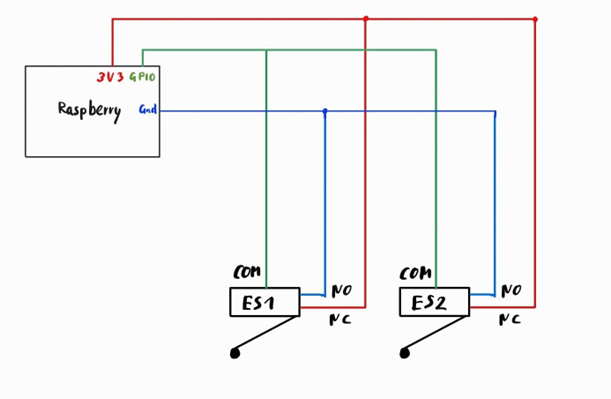
\includegraphics{image/Zusammenschaltung-Endschalter.png}
    \caption{Zusammenschaltung Endschalter}
    \label{fig:enter-label}
\end{figure}
Wenn die Teststation während einem Test bewegt wird, könnten durch die Erschütterungen die Endschalter elektrische Störungen erkennen. Um dies zu verhindern, müssen die Endschalter mindestens eine Sekunde lang das jeweilige Signal erkennen. 
